\section{Problem Statement}
	Wind tunnels are mechanisms used for analyzing the aerodynamic properties of objects,
	that is, how these objects interact with air in motion. The mechanism simulates air in motion and
	the effect on the object is measured using a device that intercepts the forces caused by the air.
	These forces/components are denoted drag, lift and side. The drag is the horizontal force parallel
	to the direction of the air, lift is the vertical force, and side is the rotation about the vertical axis.

	The Civil Engineering Department of the University of Puerto Rico, Mayaguez Campus
	[1] has a small wind tunnel used for research. It was built around 1983 and since then has not
	been renewed to use new technology that may improve the measurements of the experiments conducted with it. The
	component that measures the forces, the balance, has a design that is completely mechanical and
	requires manual measurement of forces. Sensor data from the experiments such as temperature,
	humidity, pressure, and others are also measured manually.
	Setting an initial position using weight without the tunnel being turned on, uses the
	current mechanical balance. Once the tunnel is turned on, the balance will go out of its initial
	position. Weight is used to return the balance to its initial position and it is placed by force component
	(currently drag and lift only). Only the weight added in each component is then measured using a
	scale, and these weights represent the amount of force caused by the air.
	
	Last semester, Anthony, Jesus and Juan [2] worked in the
	Microprocessor Interfacing course on this problem and successfully implemented a design of the
	balance that used strain gauges to measure the forces, added the third component
	to the design, the side, and implemented the
	basis for using electronic sensors
	(temperature, humidity, barometric pressure, wind speed).
	
	The project while successful as proof of concept, requires scaling up and
	installation in the facility as it was developed in a prototype tunnel. Installation requires
	changing the design of some components to be adjusted to the facility and new components 
	to complete the design and provide additional functionality. The following figure shows an overview
	of the proposed system:

	\begin{figure}[H]
		\centering
			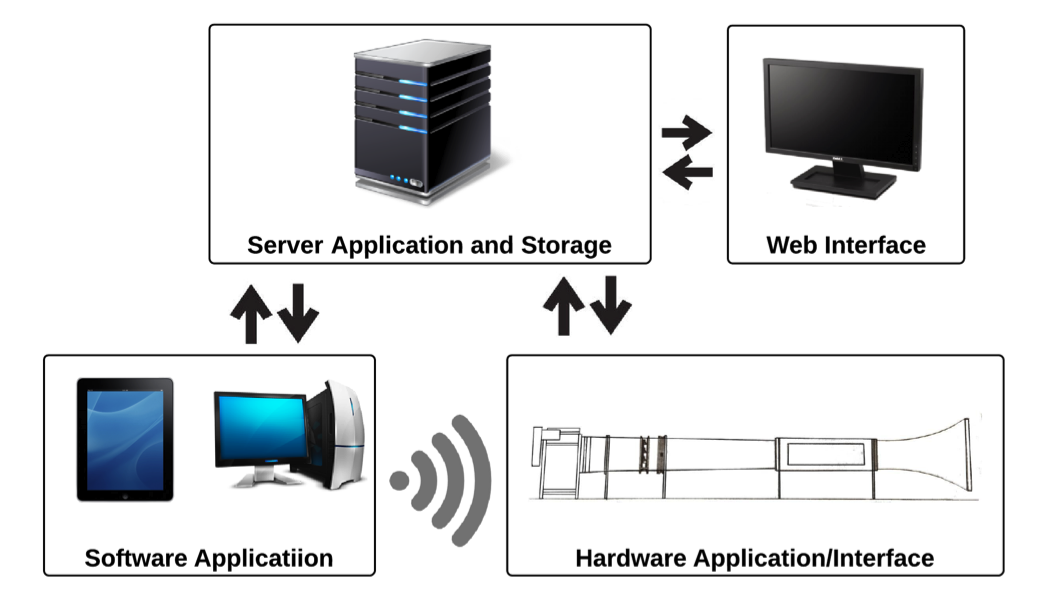
\includegraphics[scale=0.22]{img/system-overview-global}
		\caption{A global view of the proposed system.}
	\end{figure}
	
	\subsection{Installation}
	Aside from designing a new base for the balance, sensors have
	to be placed in the tunnel. A PCB will be designed to create a compact, clean, and organized
	solution that is robust and stable. The signals received from the measurement of forces require
	conditioning to eliminate noise. A power management unit has to be implemented according to
	the voltage levels used in the implementation, which was previously performed by independent
	MCUs used as power supplies.

	\subsection{Expansion}
	In order to complete the project, additional components will be implemented to allow
	easier interaction with the design at the actual wind tunnel. The current software design stores data in files, but
	does not provide visualization or statistical analysis or other calculations that can 
	be added to the system. Storage of data in
	files provides only individual analysis and if cumulative analysis is desired, it must be manually
	performed. Expanding the software to include these features may be accomplished using a
	database, and implementing the appropriate software modules. This software
	will include a user interface that has the option to use on a computer or a tablet. At the
	same time, an account control may be implemented to allow multiple users access to
	data remotely and use data history for their experiments. The third force component, the side,
	must be integrated into the measurements in the software. Data could also be delivered to other
	remote users that desire to compare results.

	As for hardware design, an interface for the wind speed window control mechanism which controls the 
	speed of the wind in the tunnel must be implemented as well as the algorithm that allows the 
	adjustment of this speed.
	An image acquisition module of the object is proposed such that the reference data of the object
	being studied can be stored along with the data captured.
